\section{Results}\label{sec:results}
This section discusses preliminary results from the analysis. Table~\ref{table:coeffs} in the appendix shows the estimated coefficients for all variables. Due to the use of factor variables, as well as a number of interaction terms, the number of estimated coefficients is very large. When estimating probability models, it is standard procedure to report estimated marginal effects of the various variables.

When independent variables are factor variables, as is the case in this analysis, then average marginal effects are computed using actual values of variables. For example, to compute the average marginal effect of preference to work, first the average predicted probability of participation of women having the preference to work is computed by inserting actual observations into the estimated regression model. Next, the same average probablity is computed for women displaying the preference to stay at home, and the marginal effect if the difference between these two estimated probabilities.

This section first discusses the etimated marginal effects of explanatory variables on and labour force participation for prime-age women in low-gap countries. This group of women could be considered as the baseline group, as young and old women probably have different constraints and motivation to participate, while women in high-gap countries, or women in developing countries, also face different constraints. Next, this section investigates how drivers of participation change in their impact for the non-baseline groups.

\subsection{Baseline results for drivers of participation}
The unconditional marginal effects of fundamental drivers reveal that for prime-age women in low gap countries, the group with the least amount of constraints, their preference to work most positively increases their probability to participate in the labour market by 18 percentage points, all other factors being equal (see Figure~\ref{table:unconditional_marginal_effects}). Tertiary education has the second largest impact on the probability to participate by 13 percentage points. Whereas, partnership, children and religion has a negative affect on a prime-age women's probability to participate in the labour market among low gap countries. The negative impact of partnerships and children highlights the disproportionate care demands prime-age women face as the literature suggests. The affect of household social norms also demonstrates a significant affect on a woman's probability to participate as the household's acceptability of a woman working increases the probability by 4 percentage points. 

\begin{figure}[htb]
	\centering
	\caption{Unconditional marginal effects: prime-age women in low gap countries}
	
	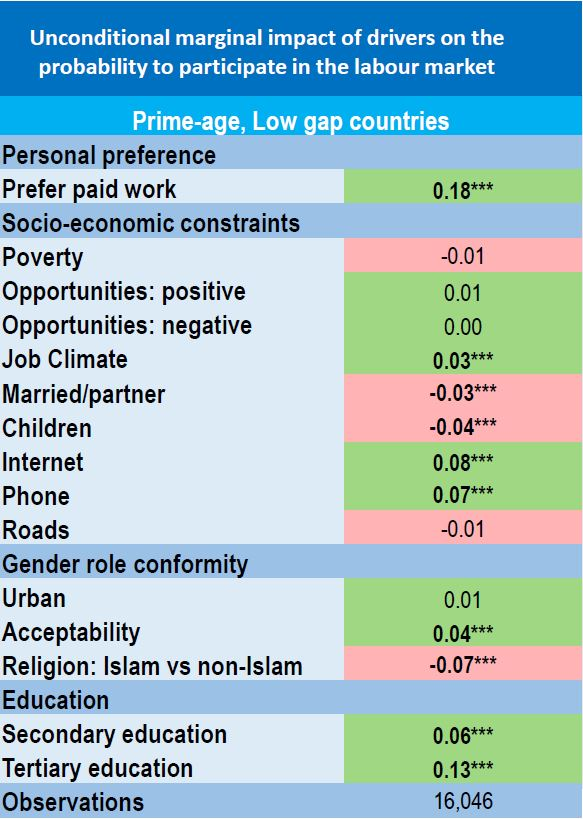
\includegraphics[width=70mm,keepaspectratio,height=0.6\textheight]{Figures/uncond_margins}
	\label{table:unconditional_marginal_effects}
\end{figure}

These baseline results highlight that a woman's participation is, among other things, very much a function of her ability to balance her role as a caregiver in the household with the demands of the workplace. A woman's role in the household and thus her preference and decision (even the freedom to choose) to participate in the labour market, are determined by social norms. The gender roles that arise from social norms vary across regions, but also vary according to the different traditional values held within different localities (urban vs rural), religions and even individual households.  

\subsection{Life-cycle effects}
To account for the various circumstances women face at different points in their lives, this section examines the differential life-cycle affects of the fundamental drivers across age groups and regions to account for the various circumstances women face at different points in their lives. 

First, the effects of socio-economic constraints on the probability to participate vary widely by age (Figure ~\ref{fig:constraints}) despite region. Poverty, for instance, follows a concave shape in effect as it increases the probability to participate for youth and even more-so for the elderly but has a slight negative affect among prime-age women. Living in an urban area has a positive affect among youth and prime-age women, but significantly reduces the probability to participate among elderly women. The perception of job opportunities has a positive affect on participation among prime and elderly but unexpectedly reduces the probability for youth. These findings highlight the varying degrees in which socio-economic constraints can affect the decision to participate for women depending on their life-cycle circumstances. 

\begin{figure}[htb]
	\centering
	\caption{Life-cycle effects: socio-economic constraints}
	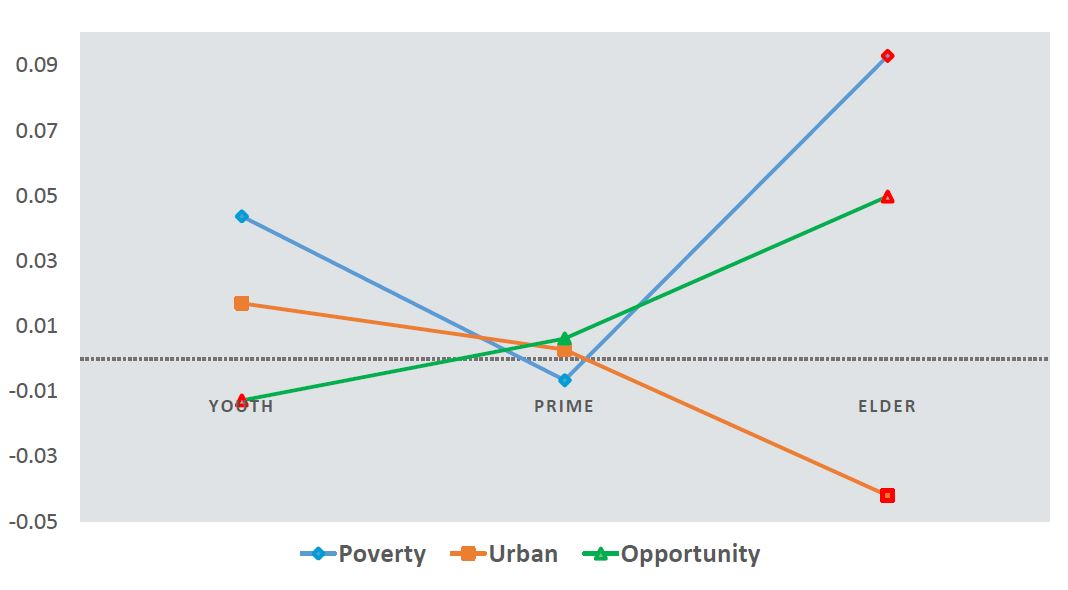
\includegraphics[width=120mm,keepaspectratio,height=0.6\textheight]{Figures/socioecon}
	\label{fig:constraints}
\end{figure}

This affect is also demonstrated by the varying challenges women face at different points in their lives, as reported in the survey, and to what extent these challenges affect their probability to participate (Figure ~\ref{fig:challenges}). Youth and prime-age women in low-gap countries most frequently report 'work and family balance' and 'abuse, harassment, and discrimination' as the biggest challenge faced in the labour market, while elderly women most frequently report 'work and family balance' and 'unequal pay'. Yet, the actual challenges that significantly affect their probability to participate differs. Youth are most significantly negatively affected by 'lack of transportation' and 'work and family balance' while for prime-age women they are most significantly negatively affected by the challenges of 'lack of transportation' and 'family members don't approve'. For elderly women, no challenges were estimated to significantly affect their probability to participate.  


\begin{figure}[htb]
	\centering
	\caption{Life-cycle effects: challenges in the labour market}
	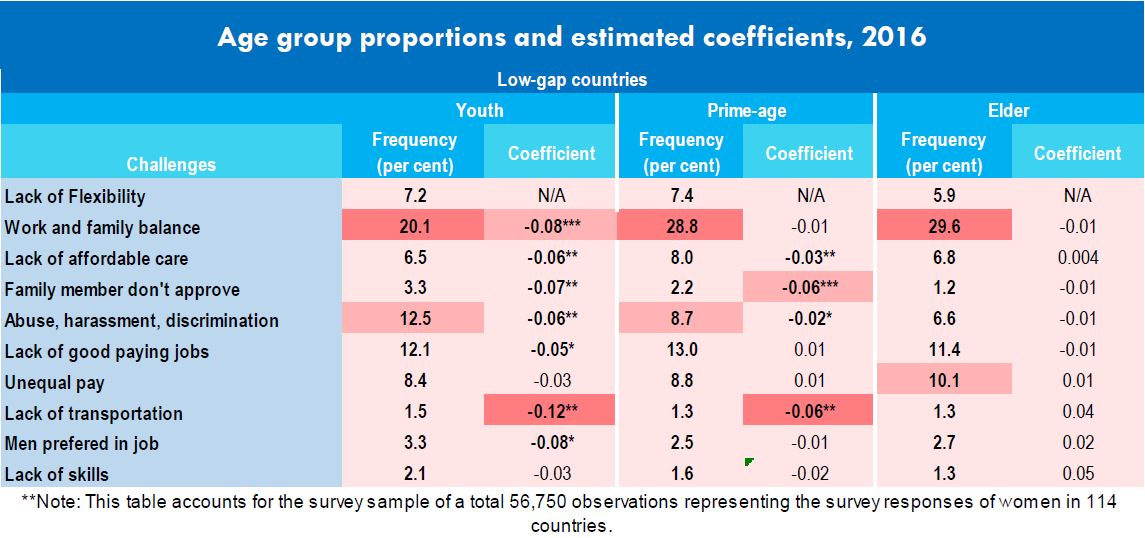
\includegraphics[width=140mm,keepaspectratio,height=0.6\textheight]{Figures/challenges}
	\label{fig:challenges}
\end{figure}

The life-cycle effects also differ across regions (Figure ~\ref{fig:marriage}). First, the general effects of partnership on the probability to participate follow a similar concave life-cycle pattern across the regions but at different magnitudes. Partnership increases the probability to participate for youth and elderly across all regions, while for prime-age women the effect is negative and to a significantly greater extent in high-gap countries. Overall, the probability to participate is higher in developing countries given the economic conditions of the region which induces a greater need to work. In general, the lower probabilities of participating among partnered prime-age women are likely due to two main reasons. The first is the economic stability that arises from a partner's income, reinforced by the 'male breadwinner' bias: the fact that the (male) 'breadwinner' is providing the household income reduces the economic imperative for a woman's labour market participation (in the case of developing countries, this effect is outweighed by economic necessity). The second and related reason is that economic stability enables social norms to confine women to more traditional roles within the household, i.e. shouldering a disproportionate burden of household responsibilities, which limits their choice and availability for paid work.

\begin{figure}[htb]
	\centering
	\caption{Life-cycle effects: partnership}
	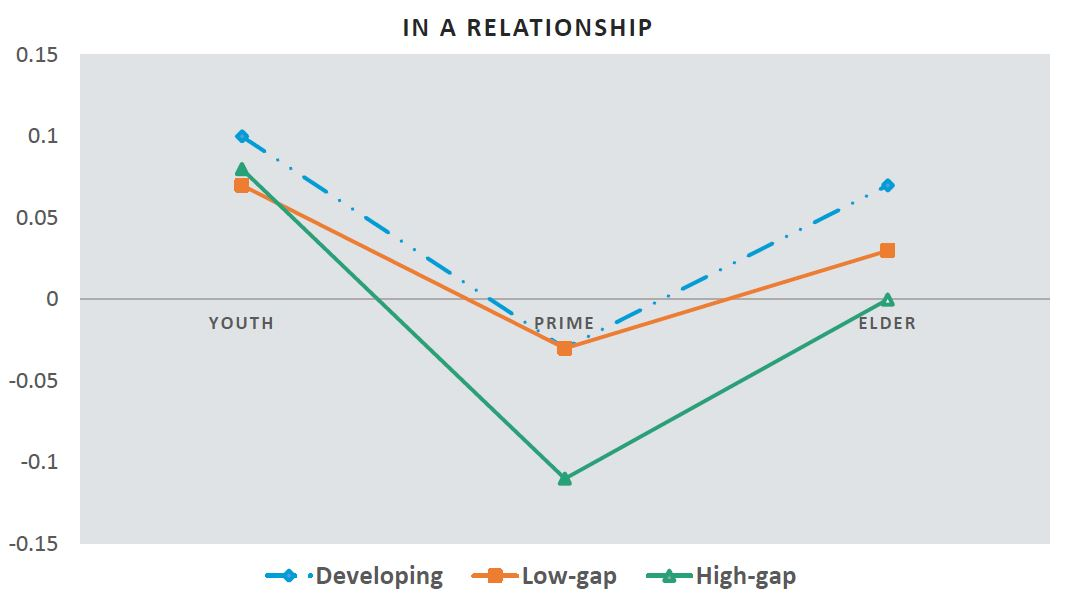
\includegraphics[width=120mm,keepaspectratio,height=0.6\textheight]{Figures/relationship}
	\label{fig:marriage}
\end{figure}

Lastly and most surprisingly, the life-cycle affects of education across the regions demonstrate divergent patterns (Figure ~\ref{fig:education} and ~\ref{fig:education2}). Youth women in developing countries face a negative probability to participate with secondary and tertiary education whereas in both low-gap and high-gap countries the affect is positive and increases for women with tertiary education. For prime-age women across all regions, both secondary and tertiary education increases the probability to work. This is similarly the case for elderly women in low-gap and high-gap countries, however, for elderly women in developing countries this increase in probability is particularly high for secondary education and negative for tertiary education. 

These results potentially suggest that the education variables for developing countries is likely to be picking up on other factors unaccounted for by the model. Hence, it is one possibility to consider that the effect of education on the probability to participate in the labour market is a function of the different weights given to the income and substitution effects. The substitution effect reflects the larger opportunity cost of staying at home as potential labour income rises with higher education, thereby encouraging participation. The income effect, in contrast, occurs when the economic needs of the family can be met with a lower rate of participation, so that more of a woman's time can be devoted to fulfilling traditional gender roles. The impact of education on participation might also capture more than just the balance between the income and substitution effects. Indeed, the level of education a woman can attain is, to a certain degree, influenced by other factors. A higher level of education could actually be an indicator that a woman's gender role and socio-economic conditions are generally more conducive to participation. In that case, the direct impact of higher education is likely to be overestimated.

\begin{figure}[htb]
	\centering
	\caption{Life-cycle effects: secondary education}
	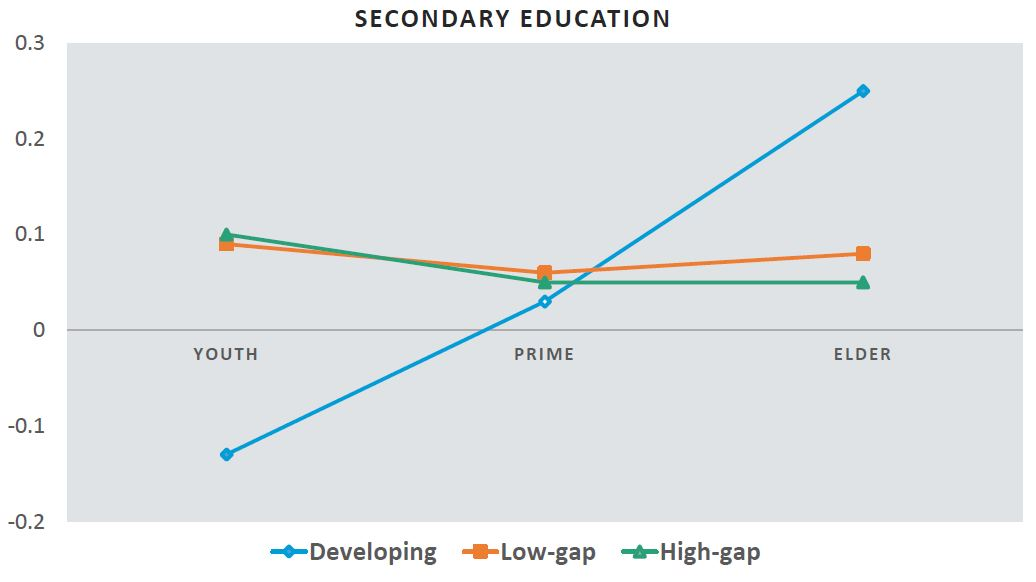
\includegraphics[width=120mm,keepaspectratio,height=0.6\textheight]{Figures/education}
	\label{fig:education}
\end{figure}

\begin{figure}[htb]
	\centering
	\caption{Life-cycle effects: tertiary education}
	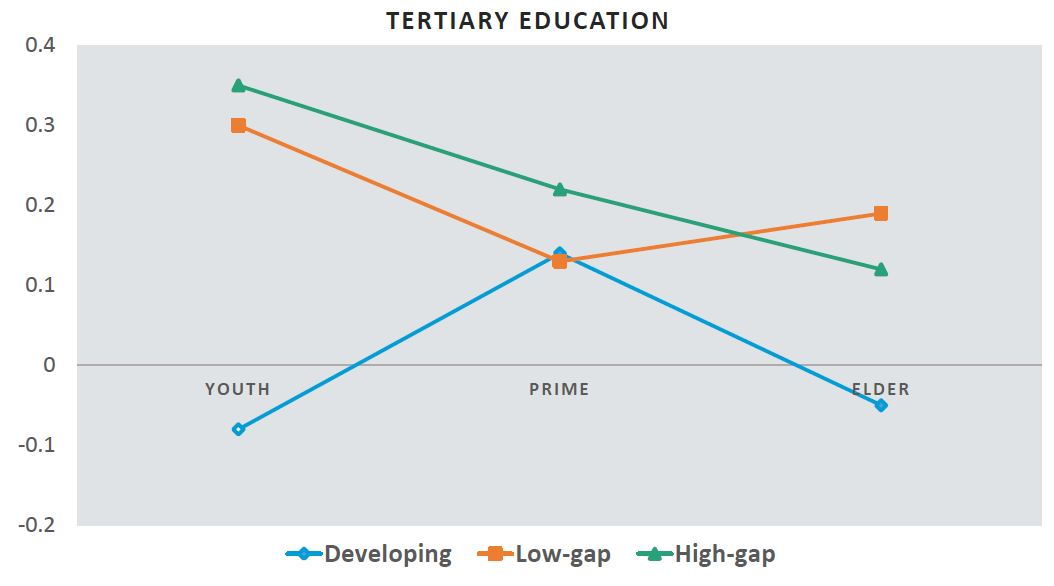
\includegraphics[width=120mm,keepaspectratio,height=0.6\textheight]{Figures/education_2}
	\label{fig:education2}
\end{figure}



\subsection{Planned future work}
For the future, some further analysis is planned. For instance, the result that poverty strongly increases the probability to participate for elderly women is very startling. One aim is to investigate whether this result varies according to the type of welfare state, providing potentially important policy conclusions.

Second, the current analysis uses the observed labour force participation gap in countries as a proxy to differentiate whether women's participation in a country is viewed favourably or not. An alternative measure would be the average response of men to the question whether women should pursue paid work form the ILO-Gallup survey. The latter has the advantage that it is a direct measure instead of a proxy, but has the disadvantage that the measure is quite noisy due to small sample size and that it only measures part of the environment that shapes women's participation. Nevertheless, it is a useful cross-check.
